\documentclass{lesson}
\pagestyle{fancy}
\fancyhf{} % 清空页眉页脚
\renewcommand{\headrulewidth}{0.4pt} % 页眉横线
\renewcommand{\footrulewidth}{0pt}   % 页脚横线
\fancyhead[C]{高二暑假物理教案}    % 页眉内容（居中）
\fancyfoot[C]{南昌学而思物理组}
\begin{document}
\section{静电场基本知识}
\concept{起电方式}{
    通过摩擦、接触和感应等方式使物体带电。\\
    常见的起电方式都遵循电荷守恒定律：在一个孤立系统内，电荷的总量保持不变，电荷既不会凭空产生，也不会凭空消失，只能从一个物体转移到另一个物体。
}
\concept{净电荷}{
    物体所带电荷的总量，正电荷和负电荷的代数和。平常所说的带电体的电荷量都是净电荷。而不是一个带电体只有正电荷或者负电荷。
}
\concept{元电荷}{
    物理学中最小的电荷量，通常用符号 $e$ 表示，约为 $1.6 \times 10^{-19} C$。该数值最早由密立根油滴实验测得，实验的原理是带电的油滴在形成的电场中，电场力等于重力时，油滴悬浮。
}
\concept{点电荷}{
    理想化的电荷模型，假设电荷集中在一个点上，具有无限小的体积。
}
\concept{电场}{
    描述电荷周围存在的一种特殊物质状态，对其他电荷产生力的作用。\\
    电场是电荷之间相互作用的媒介，任何带电体在其周围都会形成电场。\\
}
\concept{电场强度}{
    \[E=\frac Fq\]
    描述电场强弱的物理量，定义为单位正电荷在电场中所受的力。\\
    电场方向定义为该点所受的单位正电荷所受力的方向。\\
    即：电场方向总是由正电荷指向负电荷。\\
    在电场中，若放入一个正电荷，受力方向即为电场方向；若放入负电荷，受力方向与电场方向相反。
}
\concept{电场线}{
    用于表示电场方向和强度的虚构线，线的密度表示电场强度的大小。\\
    方向从正电荷指向负电荷或者无穷远，或者从无穷远指向负电荷。\\
    大小为电场线的密度，密度越大，场强越大。
}
\concept{库仑定律}{
    \[F = k \frac{|q_1 q_2|}{r^2}\]
    描述点电荷之间相互作用力的定律，其中 $k$ 为真空。\\
    库仑定律只适用于真空中静止的点电荷之间，且两电荷间的距离远大于它们自身的尺寸。
}
\newpage
\section{电势与电势能}
\concept{电势}{
    计算式为
    \[\varphi = \frac W q\]
    物体在电场中某点的电势能与该点电荷量的比值，单位为伏特（V）。
}
\notice{
    电势本身由电荷与测验点位置决定，不因电荷与电势能而影响。
}
\concept{电势差}{
    \[U=\varphi_a-\varphi_b\]
    两点之间的电势之差，类似于重力的高度差。
}
\concept{电势能}{
    \[W=\varphi q\]
    物体在电场中某点的电势能与该点电荷量的乘积，单位为焦耳（J），类似于重力势能。
}
\concept{电势能的变化}{
    \[
        \Delta W = q \Delta \varphi
    \]
    物体在电场中移动时，电势能的变化等于电荷量与电势差的乘积。
    \[
        \Delta W = W_B - W_A = q(\varphi_B - \varphi_A)
    \]
    其中 $W_A$、$W_B$ 分别为 A、B 两点的电势能，$\varphi_A$、$\varphi_B$ 分别为 A、B 两点的电势。
    \[
        W = q\varphi
    \]
    电势能等于电荷量与该点电势的乘积。
    \begin{itemize}
        \item 若 $q>0$，电荷自高电势向低电势运动，电势能减少。
        \item 若 $q<0$，电荷自低电势向高电势运动，电势能减少。
    \end{itemize}
}
\notice{
    电场力是保守力，所以其对电荷所做的功只与初末位置有关，与路径无关。
}
\newpage
\concept{电容器}{
    存储电能的元件，由两个导体之间隔着绝缘材料构成。\\
    平行板电容器是由两块平行放置的导体板组成，中间夹有绝缘介质。常用于研究电容器的基本性质。

    \begin{center}
    \begin{tikzpicture}[scale=1.2]
        % Draw plates
        \draw[thick] (0,0) -- (3,0);
        \draw[thick] (0,2) -- (3,2);
        % Label plates
        \node[left] at (0,2) {正极板};
        \node[left] at (0,0) {负极板};
        % Draw field lines
        \foreach \x in {0.4,0.8,1.2,1.6,2.0,2.4,2.8}
            \draw[->,blue] (\x,2) -- (\x,0);
        % Indicate distance d
        \draw[<->] (3.2,0) -- (3.2,2);
        \node[right] at (3.2,1) {$d$};
        % Indicate area S
        \draw[<->] (0,-0.3) -- (3,-0.3);
        \node at (1.5,-0.5) {$S$};
    \end{tikzpicture}
    \end{center}
}
\concept{电容}{
    描述电容器储存电能能力的物理量，定义为电容器中储存的电荷量与电压之比，单位为法拉（F）。\\
    平行板电容器的电容表达式为
    \[
    C = \varepsilon_0 \varepsilon_r \frac{S}{d}
    \]
    其中 $C$ 为电容，$\varepsilon_0$ 为真空介电常数，$\varepsilon_r$ 为介质的相对介电常数，$S$ 为极板面积，$d$ 为极板间距离。\\

    库仑定律中的系数 $k$ 与真空介电常数 $\varepsilon_0$ 的关系为
    \[
    k = \frac{1}{4\pi \varepsilon_0}
    \]
    其中 $k$ 是库仑定律中的比例常数，$\varepsilon_0$ 是真空介电常数。
}
\concept{电容器的充放电}{
    电容器的充电过程是指在外加电压作用下，电容器两极板之间积累电荷的过程；放电过程是指电容器释放储存的电能，电荷流向外部电路的过程。\\
    只有在电容器两极板间存在电势差（即外加电源或电压）时，电容器才能充电。\\
    充电过程中，电流方向为正极板流入、负极板流出，直到两极板间的电势差等于外加电压时，充电过程结束，电流为零。\\

    \textbf{充电过程中电流和电压的变化：}
    \begin{itemize}
        \item 电容器刚开始充电时，极板间电压为零，电流最大；
        \item 随着充电进行，极板间电压逐渐升高，电流逐渐减小；
        \item 当极板间电压等于外加电压时，电流减小到零，充电过程结束。
    \end{itemize}

    电容器存在击穿电压，当电压过大时电容器中间的绝缘材料就会被击穿，使得电容器被破坏。
}
\concept{电容器的能量}{
    电容器储存的电能可以用公式 $E = \frac{1}{2} C U^2=\frac12\frac {Q^2} C=\frac QU$ 表示，其中 $E$ 为电能，$C$ 为电容，$U$ 为电压。\\
}
\notice{
    电容器可以进行串并联，并联电容器，等效电容为电容器电容之和，串联电容器，等效电容规律和并联电阻相同。
}
\newpage
\section{带电粒子在电场中的运动}
\concept{直线运动}{
    带电粒子在电场中受到的力是恒定的，因此其运动轨迹为直线。
    \begin{itemize}
        \item \textbf{条件：} 电场为匀强电场，带电粒子初速度与电场方向平行或反平行。
        \item \textbf{类型：} 匀加速直线运动（若初速度与电场方向同向或反向）。
        \item \textbf{加速度表达式：}
        \[
            a = \frac{F}{m} = \frac{qE}{m}
        \]
        其中 $q$ 为粒子电荷量，$E$ 为电场强度，$m$ 为粒子质量。
    \end{itemize}
}
\concept{类平抛运动}{
    带电粒子在电场中沿水平方向以初速度 $v_0$ 运动，同时受到垂直方向的电场力作用，形成类平抛运动。\\
    \begin{center}
        \begin{tikzpicture}[scale=1.2]
            % Draw plates
            \draw[thick] (0,0) -- (5,0);
            \draw[thick] (0,3) -- (5,3);
            % Label plates
            \node[left] at (0,3) {正极板};
            \node[left] at (0,0) {负极板};
    
            \coordinate (M) at (2.75, 0.5);
            \coordinate (L) at (5.5, 0.5);
            \coordinate (E) at (5, 3);
            % Draw electron trajectory (parabola)
            \draw[thick,red,->,domain=0:5.5,samples=100] plot ({\x},{0.1*\x*\x+0.5});
            % Draw electric field lines
            \foreach \x in {0.7,1.5,2.3,3.1,3.9,4.7}
                \draw[->,blue] (\x,3) -- (\x,0);
            % Draw electron at entry
            \filldraw[red] (0,0.5) circle (0.08);
            \node[below left] at (0,0.5) {电子};
            % Draw velocity vector at entry
            \draw[->,thick] (0,0.5) -- (0.8,0.5);
            \node[below] at (0.4,0.5) {$v_0$};
            \draw[dashed] (0,0.5) -- (5.5,0.5);
            \draw[dashed] (2.75, 0.5) -- (5, 3);
    
            \pic [draw, "$\theta$", angle eccentricity=1.3] { angle = L--M--E };
    
        \end{tikzpicture}
    \end{center}
    带电粒子（如电子）以初速度 $v_0$ 沿水平方向进入匀强电场，在电场力作用下做类平抛运动，从另一侧离开极板。
    \[
    \left\{
    \begin{aligned}
        v_0\tan\theta &= v_y \\
        v_y^2 &= 2\frac{qE}{m}h \\
        \tan\theta &= \frac{2h}{d}
    \end{aligned}
    \right.
    \]
}
\concept{圆周运动}{
    \begin{minipage}{0.48\textwidth}
        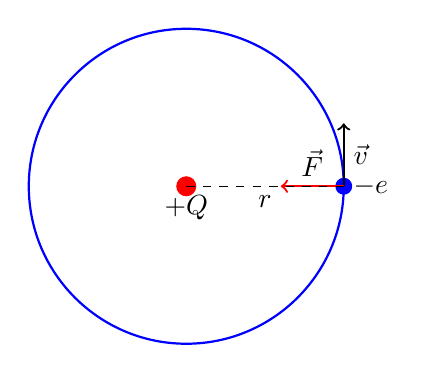
\begin{tikzpicture}[scale=1]
        % Draw central positive charge
        \filldraw[red] (0,0) circle (0.12);
        \node[below] at (0,0) {$+Q$};
        % Draw circular orbit
        \draw[thick,blue] (0,0) circle (2);
        % Draw electron on orbit
        \filldraw[blue] (2,0) circle (0.10);
        \node[right] at (2,0) {$-e$};
        % Draw velocity vector (tangent)
        \draw[->,thick] (2,0) -- (2,0.8);
        \node[right] at (2,0.4) {$\vec{v}$};
        % Draw electric force (radial)
        \draw[->,thick,red] (2,0) -- (1.2,0);
        \node[above] at (1.6,0) {$\vec{F}$};
        % Draw radius
        \draw[dashed] (0,0) -- (2,0);
        \node[below] at (1,0) {$r$};
    \end{tikzpicture}
    \end{minipage}
    \hfill
    \begin{minipage}{0.48\textwidth}
        \[F_{\text{向}}=m\frac{v^2}r=\frac{kQq}{r^2}\]
        带电粒子（如电子）在正电荷产生的电场中，在库仑力的作用下做匀速圆周运动，向心力由电场力提供。
    \end{minipage}
}
\newpage
\section{恒定电流}
\concept{电流}{
\textbf{电流的直接产生原因？}\\
载流子\underline{定向}移动。一般在金属导体中，载流子为自由电子。\\
\textbf{闭合电路的电流产生原因？}\\
电源施加电压，电压在导体两端形成电场，电场力促使自由电子定向移动。\\
\textbf{电流的方向？}\\
正电荷移动的方向，或者负电荷移动的反方向。\\
\textbf{电流的大小？}\\
单位时间内通过导体单位横截面积的电荷量为电流大小。下面是电流的定义式：
\[I=\frac Qt\]
\textbf{恒定电流？}\\
电流的大小和方向都不变的情况，并且电流仍然是一个标量，因为它没有矢量运算法则。\\
\textbf{电流的决定式：}
\[I=neSv\]
里面的n是单位体积内自由电子数量。v是自由电子的移动速度。\\
}
\notice{
    电流决定式中，面积需要垂直于移动速度的那个投影面积。
}
\concept{电阻}{
    导体中阻碍自由电子移动的情况。阻碍越严重，电阻就越大。\\
    \textbf{电阻定义式}\\
    \[R=\frac UI\]
    \textbf{电阻决定式}
    \[R=\rho\frac lS\]
    $l$是导体长度，$S$为导体的横截面积。\\
    \textbf{$\rho$电阻率影响因素？}\\
    金属类别：银<铜<铝<其他。\\
    温度，温度越大，电阻越大\\

}
\concept{电源}{
    通过非静电力做功完成电子的定向移动循环的装置。\\
    电源内部，电场力做负功，电势能增加说明必须要通过其他形式给循环输入能量，这就是非静电力，静电力是不可能完成该循环的。\\
    \textbf{电流流向}\\
    在电源外部，电流从正极流向负极。在电源的内部，电流从负极流向正极。\\
    \textbf{自由电子移动方向}\\
    自由电子从负极移动到正极，并且在正极通过非静电力回到负极。\\
    \textbf{电动势}\\
    描述电源的非静电力做功能力的物理量。数值上等于电源中非静电力将1C的电荷从负极移动到正极所做的功。\\
    \textbf{电压与电动势}\\
    电压是在电源外，电场力将自由电子从负极移动到正极的能力，而电动势是电源内部，非静电力将电子搬回负极的能力。\\
    \textbf{电源内阻}\\
    电源内部的电阻，可以认为一个电源为一个内阻与理想电源进行串联。
}
\newpage
\section{闭合电路欧姆定律}
\concept{部分电路欧姆定律}{

}
\concept{元件伏安特性曲线}{

}
\concept{串并联电路}{

}
\concept{闭合电路欧姆定律}{

}
\concept{电源伏安特性曲线}{

}
\newpage
\section{多用电表}
\newpage
\section{电源}
\newpage
\section{电路综合}
\newpage
\section{磁场}
\newpage
\section{安培力}
\newpage
\section{洛伦兹力}
\newpage
\section{带电粒子在磁场中的运动}
\newpage
\section{带电粒子在复合场中的运动}
\newpage
\section{电磁科技}
\newpage
\section{电磁感应与楞次定律}
\end{document}